\documentclass{article}
\usepackage[utf8]{inputenc}
\usepackage[margin=1in,headheight=24pt]{geometry}
\usepackage{amsmath}
\usepackage{lastpage}
\usepackage{fancyhdr}
\pagestyle{fancy}
\allowdisplaybreaks
\usepackage{graphicx}
\graphicspath{ {images/} }

\fancyhead{}
\fancyhead[L]{EGEE-2110 \\ Engineering Analysis}
\fancyhead[C]{Week 5 Homework}
\fancyhead[R]{02/19/2021 \\ Kaitlyn Wiseman}
\renewcommand{\footrulewidth}{0.4pt}
\fancyfoot{}
\fancyfoot[R]{\thepage\ of \pageref{LastPage}}


\begin{document}

{\large \noindent Problem Set:}

\par 8.3 [1, 2, 3, 4, 5]
\par 8.4 [1, 2, 9, 10]
\par 9.1 [2, 6, 22]
\par 9.2 [2, 4, 6, 8, 22, 36]
\vspace{5mm}

\noindent \hrulefill

\section*{8.3}
\setcounter{equation}{0}

\subsection*{8.3 [1]}
\setcounter{equation}{0}

Is the following matrix symmetric, skew-symmetric, or orthogonal?  Find the spectrum of the matrix, thereby illustrating Theorems 1 and 5.

\begin{align}
    \label{eq:1}
    && \textbf{A} &= \begin{bmatrix} 
    0.8 & 0.6 \\
    -0.6 & 0.8
    \end{bmatrix}
    \\
    \label{eq:2}
    && \textbf{A\textsuperscript{T}} &= \begin{bmatrix}
    0.8 & -0.6\\
    0.6 & 0.8
    \end{bmatrix}
    \\
    \label{eq:3}
    \eqref{eq:1}, \eqref{eq:2} && \textbf{AA\textsuperscript{T}} &= \begin{bmatrix}
    0.8 & 0.6 \\
    -0.6 & 0.8
    \end{bmatrix} \begin{bmatrix}
    0.8 & -0.6 \\
    0.6 & 0.8
    \end{bmatrix}
    \\
    \label{eq:4}
    && &= \begin{bmatrix}
    1 & 0\\
    0 & 1
    \end{bmatrix}
    \\
    \label{eq:5}
    && &= \textbf{I}
\end{align}

Hence, \textbf{A} is an \textbf{orthogonal} matrix.

\begin{align}
    \label{eq:6}
    \begin{vmatrix}
    \textbf{A} - \lambda\textbf{I}
    \end{vmatrix} = 0 \rightarrow && \begin{vmatrix}
    (0.8-\lambda) & 0.6\\
    -0.6 & (0.8 - \lambda)
    \end{vmatrix} &= 0
    \\
    \label{eq:7}
    && \lambda^2 -0.6\lambda +1 &= 0
    \\
    \label{eq:8}
    && \lambda_1 &= 0.8 + 0.6j
    \\
    \label{eq:9}
    && \lambda_2 &= 0.8 - 0.6j
    \\
    \label{eq:10}
    && \begin{Vmatrix} \lambda_1 \end{Vmatrix} &= 1
    \\
    \label{eq:11}
    && \begin{Vmatrix} \lambda_2 \end{Vmatrix} &= 1
\end{align}

The absolute magnitudes of each eigenvalue of this orthogonal matrix are 1, illustrating Theorem 5.

\subsection*{8.3 [2]}
\setcounter{equation}{0}

Is the following matrix symmetric, skew-symmetric, or orthogonal?  Find the spectrum of the matrix, thereby illustrating Theorems 1 and 5.

\begin{align}
    \label{eq:1}
    && \textbf{A} &= \begin{bmatrix}
        a & b\\
        -b & a
    \end{bmatrix}
    \\
    \label{eq:2}
    && \textbf{A\textsuperscript{T}} &= \begin{bmatrix}
    a & -b\\
    b & a
    \end{bmatrix}
\end{align}

\textbf{A} is symmetric iff $b = 0$, skew-symmetric iff $a = 0$.

\begin{align}
    \label{eq:3}
    && \textbf{AA\textsuperscript{T}} &= \begin{bmatrix} 
    a & b\\
    -b & a
    \end{bmatrix} \begin{bmatrix} 
    a & -b\\
    b & a
    \end{bmatrix}
    \\
    \label{eq:4}
    && &= \begin{bmatrix}
    a^2+b^2 & 0\\
    0 & a^2+b^2
    \end{bmatrix}
    \\
    \label{eq:5}
    && &= \textbf{I}
\end{align}

if $a^2+b^2=1$, making \textbf{A} orthogonal.

Find eigenvalues:

\begin{align}
    \label{eq:6}
    \begin{vmatrix}
    \textbf{A}-\lambda\textbf{I}
    \end{vmatrix} = 0 \rightarrow && \begin{vmatrix}
    (a-\lambda) & b\\
    -b & (a-\lambda)
    \end{vmatrix} &= 0
    \\
    \label{eq:7}
    && \lambda ^2 -2a \lambda +a^2 + b^2 &= 0
\end{align}

If symmetric ($b=0$):

\begin{align}
    \label{eq:8}
    && \lambda^2-2a\lambda+a^2 &= 0
    \\
    \label{eq:9}
    && (\lambda-a)^2&=0
    \\
    \label{eq:10}
    && \lambda &= a,
\end{align}

which means $a$ is real.

If skew-symmetric ($a=0$):

\begin{align}
    \label{eq:11}
    && \lambda^2 + b^2 &= 0
    \\
    \label{eq:12}
    && (\lambda + b)(\lambda - b) &= 0
    \\
    \label{eq:13}
    && \lambda &= -b, b,
\end{align}

which means $b$ is imaginary or zero.

If orthogonal ($a^2 + b^2 = 1$):

\begin{align}
    \label{eq:14}
    && \lambda^2 - 2a\lambda + 1 &= 0
    \\
    \label{eq:15}
    \text{If } \begin{Vmatrix}
    a
    \end{Vmatrix} = 1: && \lambda^2 - 2a\lambda + a^2 &= 0
    \\
    \label{eq:16}
    &&(\lambda-a)^2 &= 0
    \\
    \label{eq:17}
    &&\lambda &= a
    \\
    \label{eq:18}
    &&\begin{Vmatrix}
    \lambda
    \end{Vmatrix} &= 1,
\end{align}

illustrating Theorem 5.

\subsection*{8.3 [3]}
\setcounter{equation}{0}

Is the following matrix symmetric, skew-symmetric, or orthogonal?  Find the spectrum, illustrating Theorems 1 and 5.

\begin{align}
    \label{eq:1}
    && \textbf{A} &= \begin{bmatrix}
    2 & 8\\
    -8 & 2
    \end{bmatrix}
    \\
    \label{eq:2}
    && \textbf{A\textsuperscript{T}} &= \begin{bmatrix}
    2 & -8\\
    -8 & 2
    \end{bmatrix} \neq \textbf{A}, -\textbf{A}
    \\
    \label{eq:3}
    && \textbf{AA\textsuperscript{T}} &= \begin{bmatrix}
    2 & 8\\
    -8 & 2 \end{bmatrix} \begin{bmatrix} 
    2 & -8 \\
    8 & 2 \end{bmatrix}
    \\
    \label{eq:4}
    && &= \begin{bmatrix} 68 & 0 \\ 0 & 68 \end{bmatrix} \neq \textbf{I}
\end{align}

\textbf{A} is not symmetric, skew-symmetric, or orthogonal.  Find eigenvalues:

\begin{align}
    \label{eq:5}
    \begin{vmatrix}
    \textbf{A} - \lambda \textbf{I}
    \end{vmatrix} 0 && \begin{vmatrix}
    (2-\lambda) & 8\\
    -8 & (2-\lambda)
    \end{vmatrix} &= 0
    \\
    \label{eq:6}
    && \lambda^2 -4\lambda +68 &= 0
    \\
    \label{eq:7}
    && \lambda &= 2 \pm 8j
\end{align}

The eigenvalues are not real, are not purely imaginary or zero, and do not have absolute values of 1.

\subsection*{8.3 [4]}
\setcounter{equation}{0}

Is the following matrix symmetric, skew-symmetric, or orthogonal?  Find the spectrum.

\begin{align}
    \label{eq:1}
    && \textbf{A} &= \begin{bmatrix}
    \cos{\theta} & -\sin{\theta}\\
    \sin{\theta} & \cos{\theta}
    \end{bmatrix}
    \\
    \label{eq:2}
    && \textbf{A\textsuperscript{T}} &= \begin{bmatrix}
    \cos{\theta} & \sin{\theta}\\
    -\sin{\theta} & \cos{\theta}
    \end{bmatrix} \neq \textbf{A}, -\textbf{A}
    \\
    \label{eq:3}
    && \textbf{AA\textsuperscript{T}} &= \begin{bmatrix}
    \cos{\theta} & -\sin{\theta}\\
    \sin{\theta} & \cos{\theta}
    \end{bmatrix} \begin{bmatrix}
    \cos{\theta} & \sin{\theta}\\
    -\sin{\theta} & \cos{\theta}
    \end{bmatrix}
    \\
    \label{eq:4}
    && &= \begin{bmatrix}
    (\cos^2 \theta + \sin^2 \theta) & (\cos{\theta}\sin{\theta} - \cos{\theta}\sin{\theta})\\
    (\sin{\theta}\cos{\theta} - \sin{\theta}\cos{\theta}) & (\sin^2 \theta + \cos^2 \theta)
    \end{bmatrix}
    \\
    \label{eq:5}
    && &= \begin{bmatrix}
    1 & 0\\
    0 & 1
    \end{bmatrix} = \textbf{I}
\end{align}

Hence, \textbf{A} is orthogonal.  Find the eigenvalues:

\begin{align}
    \label{eq:6}
    \begin{vmatrix} \textbf{A} - \lambda\textbf{I}\end{vmatrix} = 0: &&\begin{vmatrix} 
    (\cos\theta - \lambda) & -\sin\theta\\
    \sin\theta & (\cos\theta - \lambda)
    \end{vmatrix} &= 0
    \\
    \label{eq:7}
    && \lambda^2 -(2\cos\theta)\lambda + 1 &= 0
    \\
    \label{eq:8}
    && \lambda &= \cos\theta \pm (\sin\theta)j
    \\
    \label{eq:9}
    && \begin{Vmatrix} \lambda \end{Vmatrix} &= \sqrt{\cos^2 \theta + \sin^2 \theta}
    \\
    \label{eq:10}
    && &= 1
\end{align}

The eigenvalues have an absolute value of 1, illustrating Theorem 5 (that the eigenvalues of orthogonal matrices have absolute values of 1).

\subsection*{8.3 [5]}
\setcounter{equation}{0}

Is the following matrix symmetric, skew-symmetric, or orthogonal?  Find the spectrum.

\begin{align}
    \label{eq:1}
    && \textbf{A} &= \begin{bmatrix}
    6 & 0 & 0\\
    0 & 2 & -2\\
    0 & -2 & 5
    \end{bmatrix}
    \\
    \label{eq:2}
    && \textbf{A\textsuperscript{T}} &= \begin{bmatrix}
    6 & 0 & 0\\
    0 & 2 & -2\\
    0 & -2 & 5
    \end{bmatrix} = \textbf{A}
\end{align}

Hence, \textbf{A} is symmetric.  Find the eigenvalues:

\begin{align}
    \label{eq:3}
    \begin{vmatrix}
    \textbf{A} - \lambda\textbf{I}
    \end{vmatrix} = 0: && \begin{bmatrix}
    (6-\lambda) & 0 & 0\\
    0 & (2-\lambda) & -2\\
    0 & -2 & (5-\lambda)
    \end{bmatrix} &= 0
    \\
    \label{eq:4}
    && -\lambda^3 + 13\lambda^2 -48\lambda + 36 &= 0
    \\
    \label{eq:5}
    \text{from MATLAB}: && \lambda &= 6, 6, 1
\end{align}

All eigenvalues are real, illustrating Theorem 1.

\newpage

\section*{8.4}
\setcounter{equation}{0}

\subsection*{8.4 [1]}
\setcounter{equation}{0}

Verify that \textbf{A} and \textbf{$\hat{\text{A}} = \textbf{P}^{-1} \textbf{A} \textbf{P}$} have equal eigenvalues.  If \textbf{y} is an eigenvector of \textbf{$\hat{\text{A}}$} and \textbf{x} an eigenvector of \textbf{A}, show that $\textbf{x}=\textbf{Py}$.

\begin{align}
    \label{eq:1}
    && \textbf{A} = \begin{bmatrix} 3&4\\4&-3\end{bmatrix} &\text{,  } \textbf{P} = \begin{bmatrix} -4&2\\3&-1\end{bmatrix}
    \\
    \label{eq:2}
    && \det{\textbf{P}} &= -2 \neq 0
    \\
    \label{eq:3}
    && \textbf{P}^{-1} &= \frac{1}{\det\textbf{P}}\textbf{C\textsuperscript{T}}
    \\
    \label{eq:4}
    && &= -\frac{1}{2}\begin{bmatrix} -1 & -2\\-3 & -4 \end{bmatrix}
    \\
    \label{eq:5}
    && &= \begin{bmatrix} \frac{1}{2} & 1\\ \frac{3}{2}&2 \end{bmatrix}
    \\
    \label{eq:6}
    &&\hat{\textbf{A}} &= \textbf{P}^{-1}\textbf{AP}
    \\
    \label{eq:7}
    && &= 
    \begin{bmatrix}\frac{1}{2}&1\\\frac{3}{2}&2\end{bmatrix}
    \begin{bmatrix}
    3&4\\4&-3
    \end{bmatrix}
    \begin{bmatrix}
    -4&2\\3&-1
    \end{bmatrix}
    \\
    \label{eq:8}
    && &= \begin{bmatrix}
    \frac{11}{2}&-1\\ \frac{25}{2}&0
    \end{bmatrix}\begin{bmatrix}
    -4&2\\3&-1
    \end{bmatrix}
    \\
    \label{eq:9}
    && &= \begin{bmatrix}
    -25 & 12\\ -50 & 25
    \end{bmatrix}
\end{align}

Check if \textbf{A} and $\hat{\textbf{A}}$ have the same eigenvalues:

\begin{align}
    \label{eq:10}
    \textbf{A}: \begin{vmatrix}
    \textbf{A} - \lambda\textbf{I}
    \end{vmatrix}=0 \rightarrow && \begin{vmatrix}
    (3-\lambda) & 4 \\ 4 & (-3-\lambda)
    \end{vmatrix}
    \\
    \label{eq:11}
    && \lambda^2-25 &= 0
    \\
    \label{eq:12}
    && \lambda_\textbf{A} &= \pm 5
    \\
    \label{eq:13}
    \hat{\textbf{A}}: \begin{vmatrix}
    \textbf{A} - \lambda\textbf{I}
    \end{vmatrix}=0 \rightarrow && \begin{vmatrix}
    (-25-\lambda) & 12\\
    -50 & (25-\lambda)
    \end{vmatrix} &= 0
    \\
    \label{eq:14}
    && \lambda^2 -25 &= 0
    \\
    \label{eq:15}
    && \lambda_\hat{\textbf{A}} &= \pm 5 = \lambda_\textbf{A}
\end{align}

$\hat{\textbf{A}}$ and \textbf{A} have the same eigenvalues.  Find eigenvectors of \textbf{A}:

\begin{align}
    \label{eq:16}
    \lambda_\textbf{A} = 5: && \begin{bmatrix}
    (3-5) & 4\\4&(-3-5)
    \end{bmatrix} \textbf{x}_{\lambda_\textbf{A} = 5} &= \textbf{0}
    \\
    \label{eq:17}
    &&\begin{bmatrix}
    -2 & 4 &|& 0\\
    4&-8 &|& 0
    \end{bmatrix}
    \\
    \label{eq:18}
    \textbf{R}_2 = \textbf{R}_2 +2\textbf{R}_1 \rightarrow && \begin{bmatrix}
    -2 & 4 &|& 0\\
    0 & 0 &|& 0
    \end{bmatrix}
    \\
    \label{eq:19}
    && 2x_1 &= 4x_2
    \\
    \label{eq:20}
    && x_1 = 2 &, x_2 = 1
    \\
    \label{eq:21}
    && \textbf{x}_{\lambda_\textbf{A}=5} &= \begin{bmatrix}
    2\\1
    \end{bmatrix}
    \\
    \label{eq:22}
    \lambda_\textbf{A} = -5: && 
    \begin{bmatrix}
    (3+5) & 4\\
    4 & (-3+5)\end{bmatrix} \textbf{x}_{\lambda_\textbf{A}=-5} &= \textbf{0}
    \\
    \label{eq:23} 
    && \begin{bmatrix}
    8 & 4 &|& 0\\
    4 & 2 &|& 0
    \end{bmatrix}
    \\
    \label{eq:24}
    \textbf{R}_2 = \textbf{R}_2 -\frac{1}{2}\textbf{R}_1 \rightarrow && \begin{bmatrix}
    8 & 4 &|& 0\\
    0&0&|& 0
    \end{bmatrix}
    \\
    \label{eq:25}
    && 8x_1&=-4x_2
    \\
    \label{eq:26}
    && x_1=1 &, x_2 &= -2
    \\
    \label{eq:27}
    && \textbf{x}_{\lambda_\textbf{A} = -5} &= \begin{bmatrix}
    1\\-2
    \end{bmatrix}
\end{align}

Find eigenvectors of $\hat{\textbf{A}}$:

\begin{align}
    \label{eq:28}
    \lambda_{\hat{\textbf{A}}} = 5: && \begin{bmatrix}
    (-25-5) & 12\\
    -50 & (25-5)
    \end{bmatrix} \textbf{x}_{\lambda_{\hat{\textbf{A}}} = 5} &= \textbf{0}
    \\
    \label{eq:29}
    && \begin{bmatrix}
    -30 & 12 &|& 0\\
    -50 & 20 &|& 0
    \end{bmatrix}
    \\ 
    \label{eq:30}
    \textbf{R}_2 = \textbf{R}_2 -\frac{5}{3}\textbf{R}_1 \rightarrow && \begin{bmatrix}
    -30 & 12 &|& 0\\
    0 & 0 &|& 0
    \end{bmatrix}
    \\
    \label{eq:31}
    && 30x_1 &= 12x_2
    \\
    \label{eq:32}
    && x_2 = 5 &, x_1 = 2
    \\
    \label{eq:33}
    && \textbf{x}_{\hat{\lambda} = 5} &= \begin{bmatrix}
    2\\5
    \end{bmatrix}
    \\
    \label{eq:34}
    \hat{\lambda}=-5: && \begin{bmatrix}
    (-25+5) & 12\\
    -50 & (25+5)
    \end{bmatrix} \textbf{x}_{\hat{\lambda}=-5} &= \textbf{0}
    \\
    \label{eq:35}
    &&\begin{bmatrix}
    -20 & 12 &|& 0\\
    -50 & 30 &|& 0
    \end{bmatrix}
    \\
    \label{eq:36}
    \textbf{R}_2 = \textbf{R}_2 - \frac{5}{2}\textbf{R}_1 \rightarrow && \begin{bmatrix}
    -20 & 12 &|& 0\\
    0 & 0 &|& 0
    \end{bmatrix}
    \\
    \label{eq:37}
    && 20x_1 &= 12x_2
    \\
    \label{eq:38}
    && x_1 = 3 &, x_2 = 5
    \\
    \label{eq:39}
    && \textbf{x}_{\hat{\lambda}=-5} &= \begin{bmatrix}
    3 \\ 5
    \end{bmatrix}
\end{align}

Show that $\textbf{x}=\textbf{Py}$, where \textbf{x} is an eigenvector of \textbf{A}, and \textbf{y} is the corresponding eigenvector of $\hat{\textbf{A}}$:

\begin{align}
    \label{eq:40}
    \lambda = 5 \rightarrow \textbf{x} = \textbf{Py}: 
    && \textbf{x}_{\lambda = 5} &= \begin{bmatrix}
    -4 & 2\\ 3 & -1
    \end{bmatrix} \begin{bmatrix} 2\\5 \end{bmatrix}
    \\
    \label{eq:41}
    && &= \begin{bmatrix}
    2\\1
    \end{bmatrix} \rightarrow \eqref{eq:21}
    \\
    \label{eq:42}
    \lambda = -5 \rightarrow \textbf{x} = \textbf{Py}: && 
    \textbf{x}_{\lambda=-5} &= \begin{bmatrix}
    -4 & 2\\ 3 & -1
    \end{bmatrix} \begin{bmatrix}
    3\\5
    \end{bmatrix}
    \\
    \label{eq:43}
    && &= \begin{bmatrix}
    -2 \\ 4
    \end{bmatrix} \rightarrow \text{a scalar multiple of } \eqref{eq:27} 
\end{align}

Hence, $\textbf{x}=\textbf{Py}$, where \textbf{x} is an eigenvector of \textbf{A}, and \textbf{y} is the corresponding eigenvector of $\hat{\textbf{A}}$.

\subsection*{8.4 [2]}
\setcounter{equation}{0}

Verify that \textbf{A} and \textbf{$\hat{\text{A}} = \textbf{P}^{-1} \textbf{A} \textbf{P}$} have equal eigenvalues.  If $\hat{\textbf{x}}$ is an eigenvector of \textbf{$\hat{\text{A}}$} and \textbf{x} an eigenvector of \textbf{A}, show that $\textbf{x}=\textbf{P}\hat{\textbf{x}}$.

\begin{align}
    \label{eq:1}
    && \textbf{A} = \begin{bmatrix}
    1&0 \\ 2 & -1
    \end{bmatrix}, \textbf{P} &= \begin{bmatrix} 7 & -5\\ 10 & -7 \end{bmatrix}
    \\
    \label{eq:2}
    && \det\textbf{P} &= 1 \neq 0
    \\
    \label{eq:3}
    && \textbf{P}^{-1} &= \frac{1}{\det\textbf{P}}\textbf{C\textsuperscript{T}}
    \\
    \label{eq:4}
    && &= \begin{bmatrix}
    -7 & 5\\
    -10 & 7
    \end{bmatrix}
    \\
    \label{eq:5}
    && \hat{\textbf{A}} &= \textbf{P}^{-1} \textbf{AP}
    \\
    \label{eq:6}
    && &= \begin{bmatrix}
    -7 & 5\\
    -10 & 7
    \end{bmatrix} \begin{bmatrix}
    1&0 \\ 2 & -1
    \end{bmatrix} \begin{bmatrix} 7 & -5\\ 10 & -7 \end{bmatrix}
    \\
    \label{eq:7}
    && &= \begin{bmatrix}
    3 & -5\\ 4 & -7
    \end{bmatrix} \begin{bmatrix} 7 & -5\\ 10 & -7 \end{bmatrix}
    \\
    \label{eq:8}
    && &= \begin{bmatrix}
    -29 & 20\\
    -42 & 29
    \end{bmatrix}
\end{align}

Find eigenvalues $\lambda$ of \textbf{A}:

\begin{align}
    \label{eq:9}
    \begin{vmatrix}
    \textbf{A} - \lambda\textbf{I}
    \end{vmatrix} = 0
    && \begin{vmatrix}
    (1-\lambda) & 0\\ 2 & (-1-\lambda)
    \end{vmatrix} &= 0
    \\
    \label{eq:10}
    && (\lambda+1)(\lambda-1) &= 0
    \\
    \label{eq:11}
    && \lambda &= \pm 1
\end{align}

Find eigenvalues $\hat{\lambda}$ of $\hat{\textbf{A}}$:

\begin{align}
    \label{eq:12}
    \begin{vmatrix}
    \textbf{A} - \lambda\textbf{I}
    \end{vmatrix} = 0 && \begin{vmatrix}
    (-29-\hat\lambda) & 20 \\
    -42 & (29 - \hat\lambda)
    \end{vmatrix} &= 0
    \\
    \label{eq:13}
    && \hat\lambda^2 -1 &= 0
    \\
    \label{eq:14}
    && \hat\lambda &= \pm 1 = \lambda
\end{align}

Hence, the eigenvalues $\lambda$ and $\hat\lambda$ of \textbf{A} and $\hat{\textbf{A}}$ are equal.  

Find eigenvectors $\textbf{x}_\lambda$ of \textbf{A}:

\begin{align}
    \label{eq:15}
    \lambda = 1: && \begin{bmatrix}
    (1-1) & 0\\
    2 & (-1-1)
    \end{bmatrix} \textbf{x}_1 &= \textbf{0}
    \\
    \label{eq:16}
    && \begin{bmatrix}
    0 & 0 &|& 0\\
    2 & -2 &|& 0
    \end{bmatrix}
    \\
    \label{eq:17}
    && 2x_1 &= 2x_2
    \\
    \label{eq:18}
    && x_1 =1 &, x_2 = 1
    \\
    \label{eq:19}
    && \textbf{x}_1 &= \begin{bmatrix}
    1\\1
    \end{bmatrix}
    \\
    \label{eq:20}
    \lambda = -1: && \begin{bmatrix}
    (1+1) & 0\\
    2 & (-1+1)
    \end{bmatrix} \textbf{x}_{-1} &= \textbf{0}
    \\
    \label{eq:21}
    &&\begin{bmatrix}
    2&0&|&0\\
    2&0&|&0
    \end{bmatrix}
    \\
    \label{eq:22}
    && x_1 = 0 &, x_2 = 1
    \\
    \label{eq:23}
    && \textbf{x}_{-1} &= \begin{bmatrix}
    0\\1
    \end{bmatrix}
\end{align}

Find eigenvectors $\hat{\textbf{x}}$ of $\hat{\textbf{A}}$:

\begin{align}
    \label{eq:24}
    \hat\lambda = 1: &&
    \begin{bmatrix}
    (-29-1) & 20\\
    -42 & (29-1)
    \end{bmatrix} \hat{\textbf{x}}_1 &= \textbf{0}
    \\
    \label{eq:25}
    && \begin{bmatrix}
    -30 & 20 &|& 0\\
    -42 & 28 &|& 0
    \end{bmatrix}
    \\
    \label{eq:26}
    \textbf{R}_2 = \textbf{R}_2 - \frac{42}{30}\textbf{R}_1 \rightarrow && \begin{bmatrix}
    -30 & 20 &|& 0\\
    0 & 0 &|& 0
    \end{bmatrix}
    \\
    \label{eq:27}
    && 30x_1 &= 20 x_2
    \\
    \label{eq:28}
    && x_1 = 2 &, x_2 = 3
    \\
    \label{eq:29}
    \hat\lambda = -1: && \begin{bmatrix}
    (-29 + 1) & 20 \\
    -42 & (29+1) 
    \end{bmatrix} \hat{\textbf{x}}_{-1} &= \textbf{0}
    \\
    \label{eq:30}
    && \begin{bmatrix}
    -28 & 20 &|& 0\\
    -42 & 30 &|& 0
    \end{bmatrix}
    \\
    \label{eq:31}
    \textbf{R}_2 = \textbf{R}_2 - \frac{42}{28}\textbf{R}_1 \rightarrow && \begin{bmatrix}
    -28 & 20 &|& 0\\
    0 & 0 &|& 0
    \end{bmatrix}
    \\
    \label{eq:32}
    && 28x_1 &= 20 x_2
    \\
    \label{eq:33}
    && x_1 = 5, x_2 &= 7
    \\
    \label{eq:34}
    && \hat{\textbf{x}}_{-1} &= \begin{bmatrix}
    5\\7
    \end{bmatrix}
\end{align}

Check that \textbf{x} $=$ \textbf{P}$\hat{\textbf{x}}$:

\begin{align}
    \label{eq:35}
    \text{For } \lambda, \hat\lambda = 1: &&
    \textbf{x}_1 &= \textbf{P} \hat{\textbf{x}}_1
    \\
    \label{eq:36}
    && &= \begin{bmatrix}
    7 & -5\\
    10 & -7
    \end{bmatrix} \begin{bmatrix}
    2 \\3
    \end{bmatrix}
    \\
    \label{eq:37} &&
    &= \begin{bmatrix}
    -1\\-1
    \end{bmatrix} \rightarrow \text{ a scalar multiple of } \eqref{eq:19}
    \\
    \label{eq:38}
    \text{For } \lambda, \hat\lambda = -1:
    && \textbf{x}_{-1} &= \textbf{P}\hat{\textbf{x}}_{-1}
    \\
    \label{eq:39}
    && &= \begin{bmatrix}
    7 & -5\\
    10 & -7
    \end{bmatrix} \begin{bmatrix}
    5\\7
    \end{bmatrix}
    \\
    \label{eq:40}
    && &= \begin{bmatrix}
    0\\1
    \end{bmatrix} \rightarrow \eqref{eq:23}
\end{align}

Hence, \textbf{x} $=$ \textbf{P}$\hat{\textbf{x}}$.

\subsection*{8.4 [9]}
\setcounter{equation}{0}

Find an eigenbasis and diagonalize.

\begin{align}
    \label{eq:1}
    && \textbf{A} &= \begin{bmatrix}
    1&2\\2&4
    \end{bmatrix}
\end{align}

Find $\lambda$'s:

\begin{align}
    \label{eq:2}
    \begin{vmatrix}
    \textbf{A} - \lambda\textbf{I}
    \end{vmatrix} = 0: && \begin{vmatrix}
    (1-\lambda) & 2\\ 2 & (4-\lambda)
    \end{vmatrix} &=0
    \\
    \label{eq:3}
    && \lambda^2-5\lambda&=0
    \\
    \label{eq:4}
    && \lambda &= 0, 5
\end{align}

Find eigenvectors:

\begin{align}
    \label{eq:5}
    \lambda = 0: && \begin{bmatrix}
    1&2\\2&4
    \end{bmatrix}\textbf{x}_0 &= \textbf{0}
    \\
    \label{eq:6}
    &&\begin{bmatrix}
    1&2 &|& 0\\
    2&4 &|& 0
    \end{bmatrix}
    \\
    \label{eq:7}
    \textbf{R}_2 = \textbf{R}_2 -2\textbf{R}_1 \rightarrow && \begin{bmatrix}
    1 & 2 &|& 0\\
    0 & 0 &|& 0
    \end{bmatrix}
    \\
    \label{eq:8}
    && x_1 &= -2x_2
    \\
    \label{eq:9}
    && x_1=-2, x_2 &= 1
    \\
    \label{eq:10}
    && \textbf{x}_0 &= \begin{bmatrix}
    -2\\1
    \end{bmatrix}
    \\
    \label{eq:11}
    \lambda = 5: && \begin{bmatrix}
    (1-5) & 2\\
    2 & (4-5)
    \end{bmatrix} \textbf{x}_5 &= \textbf{0}
    \\
    \label{eq:12}
    && \begin{bmatrix}
    -4 & 2 &|& 0\\
    2 & -1 &|& 0
    \end{bmatrix}
    \\
    \label{eq:13}
    \textbf{R}_2 = \textbf{R}_2 + \frac{1}{2}\textbf{R}_1 \rightarrow && \begin{bmatrix}
    -4 & 2 &|& 0\\
    0 & 0 &|& 0
    \end{bmatrix}
    \\
    \label{eq:14}
    && 4x_1 &= 2x_2
    \\
    \label{eq:15}
    && x_1 = 1, x_2 &= 2
    \\
    \label{eq:16}
    && \textbf{x}_5 &= \begin{bmatrix}
    1\\2
    \end{bmatrix}
\end{align}

Hence, an eigenbasis of \textbf{A} is given by

\begin{align}
    \label{eq:17}
    && \textbf{X} &= \begin{bmatrix}
    -2 & 1\\
    1 & 2
    \end{bmatrix}
\end{align}

Find \textbf{X}\textsuperscript{-1}:

\begin{align}
    \label{eq:18}
    && \textbf{X}^{-1} &= \frac{1}{\det \textbf{X}}\textbf{C\textsuperscript{T}}
    \\
    \label{eq:19}
    && \det \textbf{X} = -4-1 &= -5
    \\
    \label{eq:20}
    && \textbf{X}^{-1} &= \frac{1}{-1}\begin{bmatrix}
    2 & -1\\
    -1 & -2
    \end{bmatrix}
    \\
    \label{eq:21}
    && &= \begin{bmatrix}
    -\frac{2}{5} & \frac{1}{5}\\
    \frac{1}{5} & \frac{2}{5}
    \end{bmatrix}
\end{align}

Diagonalize \textbf{A}:

\begin{align}
    \label{eq:22}
    && \textbf{D} &= \textbf{X}^{-1}\textbf{AX}
    \\
    \label{eq:23}
    && &= \begin{bmatrix}
    -\frac{2}{5} & \frac{1}{5}\\
    \frac{1}{5} & \frac{2}{5}
    \end{bmatrix} \begin{bmatrix}
    1&2\\2&4
    \end{bmatrix} \begin{bmatrix}
    -2 & 1\\1&2
    \end{bmatrix}
    \\
    \label{eq:24}
    && &= \begin{bmatrix}
    0 & 0 \\ 1 & 2
    \end{bmatrix} \begin{bmatrix}
    -2 & 1 \\ 1 & 2
    \end{bmatrix}
    \\
    \label{eq:25}
    && &= \begin{bmatrix}
    0 & 0\\ 0 & 5
    \end{bmatrix} = \begin{bmatrix}
    \lambda_1 & 0\\
    0 & \lambda_2
    \end{bmatrix}
\end{align}

\subsection*{8.4 [10]}
\setcounter{equation}{0}

Find an eigenbasis and diagonalize.

\begin{align}
    && \textbf{A} &= \begin{bmatrix}
    1 & 0\\2&-1
    \end{bmatrix}
\end{align}

Find eigenvalues:

\begin{align}
    \begin{vmatrix}
    \textbf{A} - \lambda\textbf{I}
    \end{vmatrix}=0: && \begin{vmatrix}
    (1-\lambda) & 0\\
    2 & (-1-\lambda)
    \end{vmatrix} &= 0
    \\
    &&(1-\lambda)(-1-\lambda) &= 0
    \\
    && \lambda&= -1, 1
\end{align}

Find eigenvectors:

\begin{align}
    \lambda = -1: && \begin{bmatrix}
    (1+1) & 0\\
    2 & (-1+1)
    \end{bmatrix} \textbf{x}_{-1} &= \textbf{0}
    \\
    && \begin{bmatrix}
    2 & 0 &|& 0\\
    2 & 0 &|& 0
    \end{bmatrix}
    \\
    && x_1 = 0, x_2 &= 1
    \\
    && \textbf{x}_{-1} &= \begin{bmatrix}
    0\\1
    \end{bmatrix}
    \\
    \lambda = 1: && \begin{bmatrix}
    (1-1) & 0\\
    2 & (-1-1)
    \end{bmatrix} \textbf{x}_1 &= \textbf{0}
    \\
    &&\begin{bmatrix}
    0 & 0 &|& 0\\
    2 & -2 &|& 0
    \end{bmatrix}
    \\
    && 2x_1 &= 2x_2
    \\
    && \textbf{x}_1 &= \begin{bmatrix}
    1\\1
    \end{bmatrix}
\end{align}

Hence, an eigenbasis \textbf{X} of \textbf{A} is

\begin{align}
    && \textbf{X} &= \begin{bmatrix}
    0 & 1 \\ 1 & 1
    \end{bmatrix}
\end{align}

Find the inverse of \textbf{X}:

\begin{align}
    && \textbf{X}^{-1} &= \frac{1}{\det \textbf{X}} \textbf{C\textsuperscript{T}}
    \\
    && &= \frac{1}{-1}\begin{bmatrix}
    1 & -1\\
    -1 & 0
    \end{bmatrix}
    \\
    && &= \begin{bmatrix}
    -1 & 1\\
    1 & 0
    \end{bmatrix}
\end{align}

A diagonalization of A is thus given by

\begin{align}
    && \textbf{D} &= \textbf{X}^{-1}\textbf{AX}
    \\
    && &= \begin{bmatrix}
    -1 & 1\\
    1 & 0
    \end{bmatrix} \begin{bmatrix}
    1 & 0 \\ 2 & -1
    \end{bmatrix} \begin{bmatrix}
    0 & 1 \\ 1 & 1
    \end{bmatrix}
    \\
    && &= \begin{bmatrix}
    1 & -1\\ 1 & 0
    \end{bmatrix} \begin{bmatrix}
    0 & 1 \\ 1 & 1
    \end{bmatrix}
    \\
    && &= \begin{bmatrix}
    -1 & 0 \\ 0 & 1 
    \end{bmatrix} = \begin{bmatrix}
    \lambda_1 & 0\\ 0 & \lambda_2
    \end{bmatrix}
\end{align}

\newpage

\section*{9.1}
\setcounter{equation}{0}

\subsection*{9.1 [2]}
\setcounter{equation}{0}

Find the components of the vector \textbf{v} with initial point \textit{P} and terminal point \textit{Q}.  Find $\begin{vmatrix}
\textbf{v}
\end{vmatrix}$.  Sketch \textbf{v}.  Find the unit vector $\hat{\textbf{u}}$ in the direction of \textbf{v}.

\begin{align}
    P: (1, 1, 1)&, Q: (2, 2, 0)
    \\
    \textbf{v} &= \textbf{Q} - \textbf{P}
    \\
    &= \langle2, 2, 0\rangle - \langle1, 1, 1\rangle
    \\ 
    &= \langle1, 1, -1\rangle
    \\
    \begin{vmatrix}
    \textbf{v}
    \end{vmatrix} &= \sqrt{1^2 + 1^2 + (-1)^2}
    \\
    &= \sqrt{3}
\end{align}

Sketch of \textbf{v}:

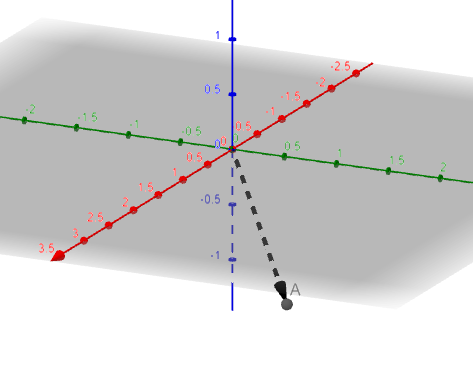
\includegraphics{9.1.2.png}

\begin{align}
    \hat{\textbf{u}} &= \frac{1}{\begin{vmatrix}
    \textbf{v}
    \end{vmatrix}} \textbf{v}
    \\
    &= \frac{1}{\sqrt{3}}\langle1, 1, -1\rangle
    \\
    &= \langle\frac{1}{\sqrt{3}}, \frac{1}{\sqrt{3}}, -\frac{1}{\sqrt{3}}\rangle
\end{align}

\subsection*{9.1 [6]}
\setcounter{equation}{0}

Find the terminal point \textit{Q} of the vector \textbf{v} with components as given and initial point \textit{P}.  Find $\begin{vmatrix}
\textbf{v}
\end{vmatrix}$.

\begin{align}
    \textbf{v} = \langle4, 0, 0\rangle &\text{    } P: (0, 2, 13)
    \\
    Q &= P + v
    \\
    &= (0, 2, 13) + (4, 0, 0)
    \\
    &= (4, 2, 13)
    \\
    \begin{vmatrix}
    \textbf{v}
    \end{vmatrix} &= \sqrt{4^2 + 0^2 + 0^2}
    \\
    &= 4
\end{align}

\subsection*{9.1 [22]}
\setcounter{equation}{0}

Find the resultant in terms of components and its magnitude.

\begin{align}
       \textbf{p} &= \langle1, -2, 3\rangle
    \\ \textbf{q} &= \langle3, 21, -16\rangle
    \\ \textbf{u} &= \langle-4, -19, 13\rangle
    \\ \textbf{r} &= \textbf{p} + \textbf{q} + \textbf{r}
    \\            &= \langle1, -2, 3\rangle + \langle3, 21, -16\rangle + \langle-4, -19, 13\rangle
    \\ &= \langle0, 0, 0\rangle
    \\
    \begin{vmatrix} \textbf{r}
    \end{vmatrix} &= 0
\end{align}

\newpage

\section*{9.2}

\subsection*{9.2 [2]}
\setcounter{equation}{0}

Given

\begin{align}
    \textbf{a} = \langle1, -3, 5\rangle && \textbf{b} = \langle4, 0, 8\rangle && \textbf{c} = \langle-2, 9, 1\rangle,
\end{align}

find

\begin{align}
    (-3\textbf{a}+5\textbf{c})\cdot\textbf{b}: && &\text{}
    (-3\langle1, -3, 5\rangle + 5\langle-2, 9, 1\rangle) \cdot \textbf{b}
    \\
    && &= (\langle-3, 9, -15\rangle + \langle-10, 45, 5\rangle) \cdot \textbf{b}
    \\
    && &= \langle-13, 54, -10\rangle \cdot \langle4, 0, 8\rangle
    \\
    && &= -13*4-10*8
    \\
    && &= -138
    \\
    15(\textbf{a}-\textbf{c}) \cdot \textbf{b}: && &\text{}
    15(\langle1, -3, 5\rangle - \langle-2, 9, 1\rangle) \cdot \textbf{b}
    \\
    && &= 15\langle3, -12, 4\rangle\cdot\langle4, 0, 8\rangle
    \\
    && &= 15(12+0+32)
    \\
    && &= 660
\end{align}

\subsection*{9.2 [4]}
\setcounter{equation}{0}

Given

\begin{align}
    \textbf{a} = \langle1, -3, 5\rangle && \textbf{b} = \langle4, 0, 8\rangle && \textbf{c} = \langle-2, 9, 1\rangle,
\end{align}

find

\begin{align}
    \begin{vmatrix}
    \textbf{a} + \textbf{b}
    \end{vmatrix}: && &\text{} \begin{vmatrix}
    \langle1, -3, 5\rangle + \langle4, 0, 8\rangle
    \end{vmatrix}
    \\
    && &= \begin{vmatrix}
    \langle5, -3, 13\rangle
    \end{vmatrix}
    \\
    && &= \sqrt{5^2 + (-13)^2 + 13^2}
    \\
    && &= \sqrt{203} \approx 14.86
    \\
    \begin{vmatrix}
    \textbf{a}
    \end{vmatrix} + \begin{vmatrix}
    \textbf{b}
    \end{vmatrix}: && &\text{} \begin{vmatrix}
    \langle1, -3, 5\rangle
    \end{vmatrix} + \begin{vmatrix}
    \langle4, 0, 8\rangle
    \end{vmatrix}
    \\
    && &= \sqrt{1^2 + (-3)^2 + 5^2} + \sqrt{4^2 + 0^2 + 8^2}
    \\
    && &= \sqrt{35} + \sqrt{80} \approx 14.25
\end{align}

\subsection*{9.2 [6]}
\setcounter{equation}{0}

Given

\begin{align}
    \textbf{a} = \langle1, -3, 5\rangle && \textbf{b} = \langle4, 0, 8\rangle && \textbf{c} = \langle-2, 9, 1\rangle,
\end{align}

find

\begin{align}
    &\begin{vmatrix}
    \textbf{a} + \textbf{c}
    \end{vmatrix}^2 + \begin{vmatrix}
    \textbf{a} - \textbf{c}
    \end{vmatrix}^2 -2 \left(\begin{vmatrix}
    \textbf{a}
    \end{vmatrix}^2 +\begin{vmatrix}
    \textbf{c}
    \end{vmatrix}^2 \right) 
    \\&= \begin{vmatrix}
    \langle1, -3, 5\rangle + \langle-2, 9, 1\rangle
    \end{vmatrix}^2 + \begin{vmatrix}
    \langle1, -3, 5\rangle - \langle-2, 9, 1\rangle
    \end{vmatrix}^2 -2 \left(1^2 + (-3)^2 + 5^2 + (-2)^2 + 9^2 +1^2\right)
    \\
    &=
    \begin{vmatrix}
    \langle-1, 6, 6\rangle
    \end{vmatrix}^2 + \begin{vmatrix}
    \langle3, -12, 4\rangle
    \end{vmatrix}^2 - 242
    \\
    &= (-1)^2 + 6^2 + 6^2 + 3^2 + (-12)^2 + 4^2 -242
    \\
    &= 0
\end{align}

\subsection*{9.2 [8]}
\setcounter{equation}{0}

Given

\begin{align}
    \textbf{a} = \langle1, -3, 5\rangle && \textbf{b} = \langle4, 0, 8\rangle && \textbf{c} = \langle-2, 9, 1\rangle,
\end{align}

find

\begin{align}
    5\textbf{a} \cdot 13\textbf{b}: && &\text{} 65\left( \langle1, -3, 5\rangle \cdot \langle4, 0, 8\rangle\right)
    \\
    && &= 65(4+0+40)
    \\
    && &= 2860
    \\
    65\textbf{a}\cdot\textbf{b}: && &= 2860
\end{align}

\subsection*{9.2 [22]}
\setcounter{equation}{0}

Find the angle between

\begin{align}
    \textbf{a} = \langle1, 1, 0\rangle, \textbf{b} &= \langle3, 2, 1\rangle 
    \\
    \cos\gamma &= \frac{\textbf{a}\cdot\textbf{b}}{\begin{vmatrix}
    \textbf{a}
    \end{vmatrix}\begin{vmatrix}
    \textbf{b}
    \end{vmatrix}}
    \\
    &= \frac{\begin{vmatrix}
    \langle1, 1, 0\rangle \cdot\langle3, 2, 1\rangle
    \end{vmatrix}}{\sqrt{2}\sqrt{14}}
    \\
    &= \frac{5}{2\sqrt{7}}
    \\
    \gamma &= \cos^{-1}\left(\frac{5}{2\sqrt{7}}\right)
    \\
    &= 0.33 \text{ rad}
\end{align}

\subsection*{9.2 [36]}
\setcounter{equation}{0}

Find the component of \textbf{a} in the direction of \textbf{b}:

\begin{align}
    \textbf{a} = \langle1, 1, 1\rangle, \textbf{b} &= \langle2, 1, 3\rangle
    \\
    p &= \textbf{a} \cdot \frac{\textbf{b}}{\begin{vmatrix}
    \textbf{b}
    \end{vmatrix}}
    \\
    &= \frac{\langle1, 1, 1\rangle \cdot \langle2, 1, 3\rangle}{\sqrt{14}} 
    \\ 
    &= \frac{6}{\sqrt{14}}
    \\
    \textbf{a}_{\textbf{b}} &= (p)\frac{\textbf{b}}{\begin{vmatrix}
    \textbf{b}
    \end{vmatrix}}
    \\
    &= \langle\frac{6}{7}, \frac{3}{7}, \frac{9}{7}\rangle
\end{align}

Make a sketch:

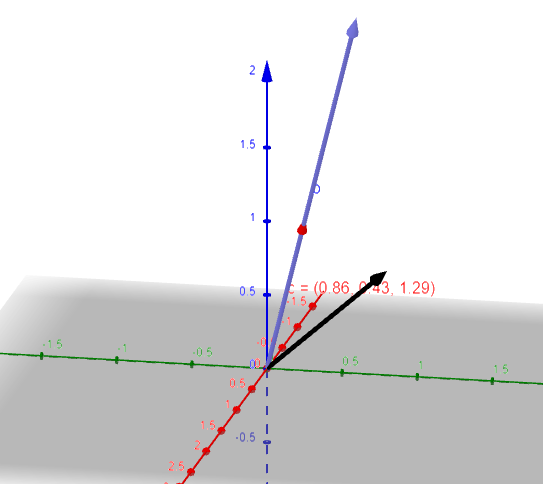
\includegraphics{9.2.36.png}

\end{document}